\documentclass[border=10pt]{standalone}
\usepackage[svgnames]{xcolor}
\usepackage{amsmath}
\usepackage{pgfplots}
\pgfplotsset{compat=newest}
\usepackage[sfdefault]{FiraSans}
\usepackage{FiraMono}
\renewcommand*\familydefault{\sfdefault}
\begin{document}
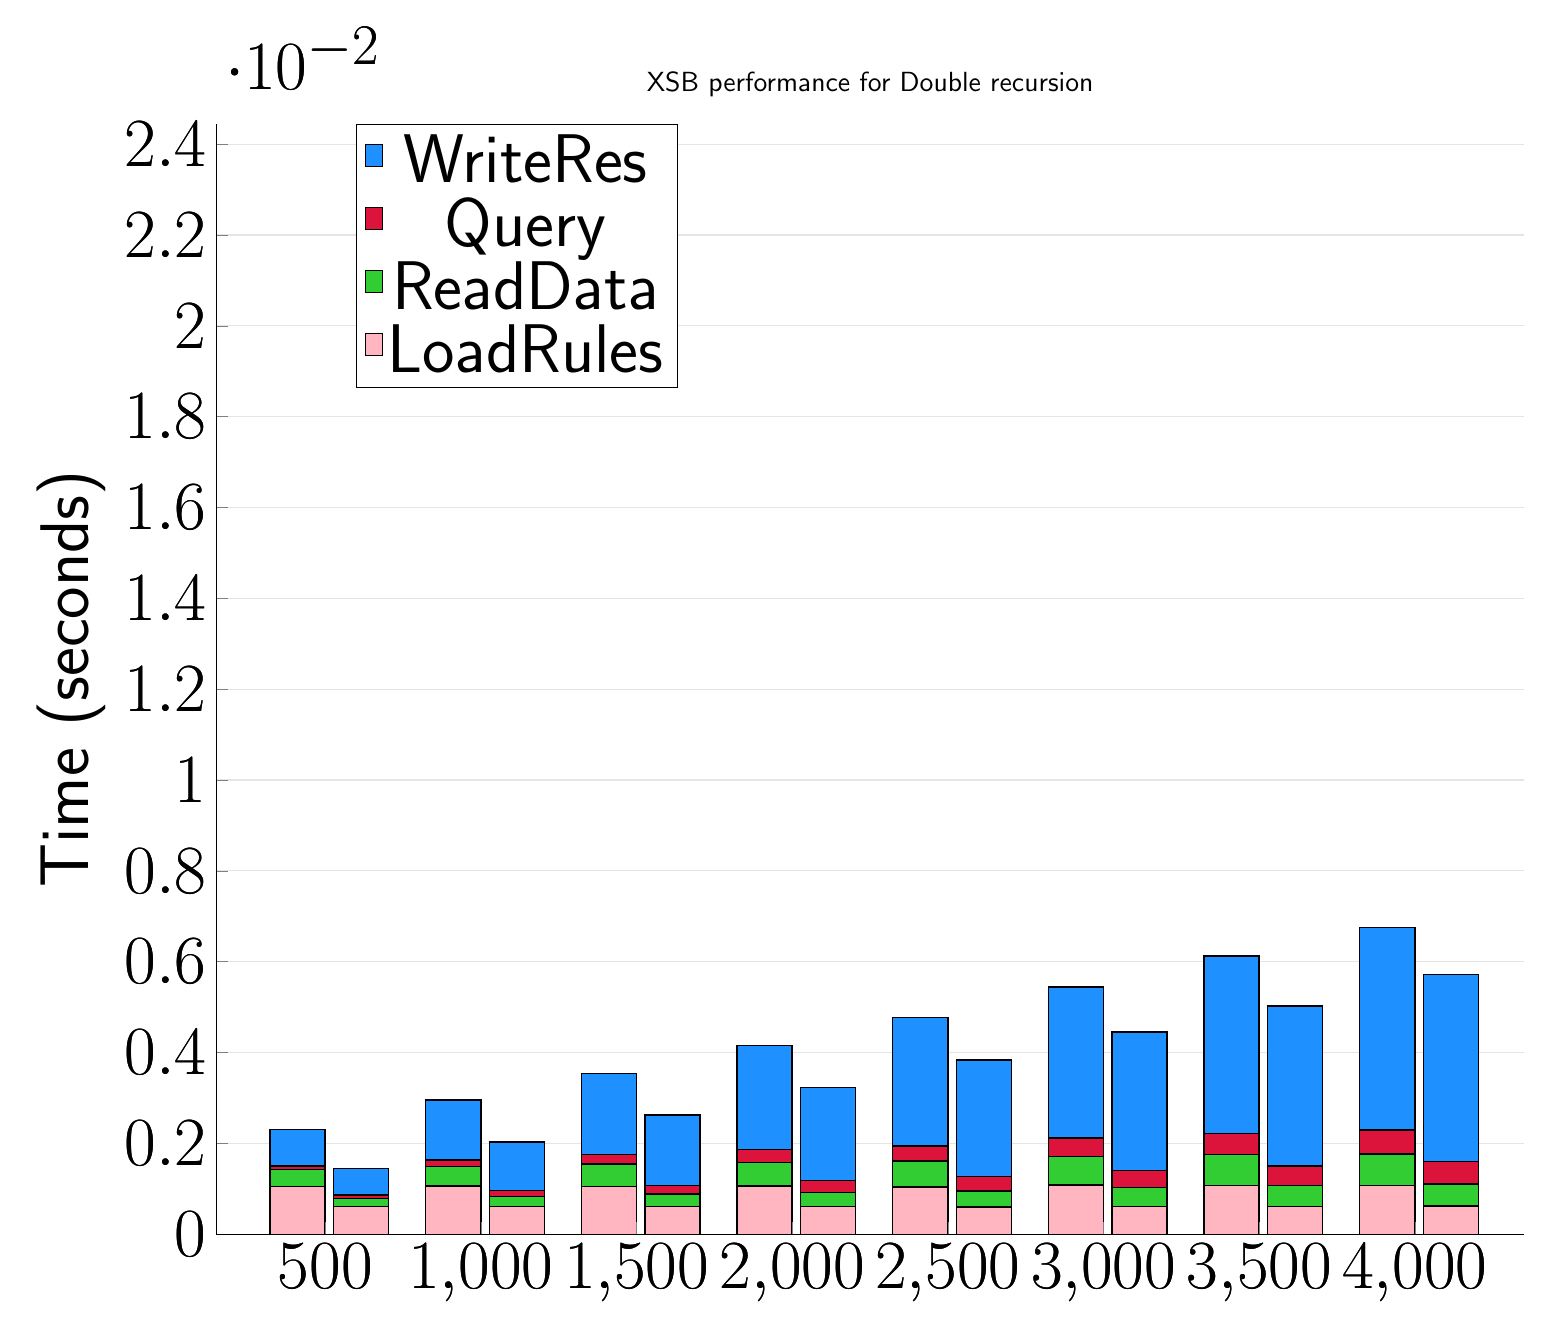
\begin{tikzpicture}
	\begin{axis}[
			ybar stacked,
			title={XSB performance for Double recursion},
			bar shift=-10pt,
			width=1.5\textwidth,
			bar width=0.7cm,
			ymajorgrids, tick align=inside,
			major grid style={draw=gray!20},
			xtick=data,
			ymin=0, ymax=0.02445413589477539,
			axis x line*=bottom,
			axis y line*=left,
			enlarge x limits=0.1,
			legend style={
					at={(0.23, 1)},
					anchor=north,
					legend columns=1,
					font=\Huge,
				},
			ylabel={Time (seconds)},
			label style={font=\Huge},
			tick label style={font=\Huge},
		]
		\addlegendimage{fill=DodgerBlue, draw=black, line width=0.2pt}
		\addlegendentry{WriteRes}
		\addlegendimage{fill=Crimson, draw=black, line width=0.2pt}
		\addlegendentry{Query}
		\addlegendimage{fill=LimeGreen, draw=black, line width=0.2pt}
		\addlegendentry{ReadData}
		\addlegendimage{fill=LightPink, draw=black, line width=0.2pt}
		\addlegendentry{LoadRules}
		\addplot +[fill=LightPink, draw=black, line width=0.5pt] coordinates {
				(500, 0.001052713394165039)
				(1000, 0.0010631799697875981)
				(1500, 0.001048636436462403)
				(2000, 0.0010582685470581052)
				(2500, 0.001043128967285156)
				(3000, 0.0010811090469360347)
				(3500, 0.001077127456665038)
				(4000, 0.0010769128799438482)
			};
		\addplot +[fill=LimeGreen, draw=black, line width=0.5pt] coordinates {
				(500, 0.0003681898117065431)
				(1000, 0.00043210983276367195)
				(1500, 0.0004941701889038087)
				(2000, 0.0005270957946777343)
				(2500, 0.000565314292907715)
				(3000, 0.0006305932998657227)
				(3500, 0.0006803274154663084)
				(4000, 0.0006886720657348633)
			};
		\addplot +[fill=Crimson, draw=black, line width=0.5pt] coordinates {
				(500, 7.903575897216796e-05)
				(1000, 0.0001425266265869139)
				(1500, 0.00020992755889892578)
				(2000, 0.0002765417098999023)
				(2500, 0.0003364801406860351)
				(3000, 0.0004029273986816406)
				(3500, 0.0004596233367919921)
				(4000, 0.0005292415618896486)
			};
		\addplot +[fill=DodgerBlue, draw=black, line width=0.5pt] coordinates {
				(500, 0.0008069276809692386)
				(1000, 0.0013206243515014651)
				(1500, 0.001788687705993652)
				(2000, 0.0022952318191528306)
				(2500, 0.0028291940689086927)
				(3000, 0.0033293724060058593)
				(3500, 0.003911399841308593)
				(4000, 0.0044541358947753915)
			};
	\end{axis}
	\begin{axis}[
			ybar stacked,
			bar shift=13pt,
			width=1.5\textwidth,
			bar width=0.7cm,
			ymajorgrids, tick align=inside,
			major grid style={draw=none},
			xtick=data,
			ymin=0, ymax=0.02445413589477539,
			axis x line*=none,
			axis y line*=none,
			enlarge x limits=0.1,
			label style={font=\Huge},
			tick label style={font=\Huge},
		]
		\addplot +[fill=LightPink, draw=black, line width=0.5pt] coordinates {
				(500, 0.0006097999999999998)
				(1000, 0.0006043000000000006)
				(1500, 0.0006052)
				(2000, 0.0006087000000000001)
				(2500, 0.0006000000000000002)
				(3000, 0.0006119999999999999)
				(3500, 0.0006163999999999999)
				(4000, 0.0006171999999999998)
			};
		\addplot +[fill=LimeGreen, draw=black, line width=0.5pt] coordinates {
				(500, 0.0001827)
				(1000, 0.00022889999999999993)
				(1500, 0.00027769999999999976)
				(2000, 0.00031620000000000015)
				(2500, 0.0003545000000000001)
				(3000, 0.0004098)
				(3500, 0.0004543000000000002)
				(4000, 0.0004874999999999999)
			};
		\addplot +[fill=Crimson, draw=black, line width=0.5pt] coordinates {
				(500, 7.27e-05)
				(1000, 0.00013309999999999968)
				(1500, 0.00019580000000000048)
				(2000, 0.0002569000000000003)
				(2500, 0.00031519999999999975)
				(3000, 0.0003746000000000002)
				(3500, 0.00042960000000000014)
				(4000, 0.0004945999999999998)
			};
		\addplot +[fill=DodgerBlue, draw=black, line width=0.5pt] coordinates {
				(500, 0.0005809)
				(1000, 0.0010615000000000004)
				(1500, 0.0015429999999999997)
				(2000, 0.0020421000000000003)
				(2500, 0.0025656000000000003)
				(3000, 0.0030565999999999996)
				(3500, 0.0035223999999999997)
				(4000, 0.004120899999999999)
			};
	\end{axis}
\end{tikzpicture}

\end{document}
